\section{Introduction}
  Poor lighting and other global conditions can reduce the quality of images. This project
  examines a few different methods of image enhancement.
  
  The first method is global histogram equalization.  Histogram equalization is especially
  useful for increasing contrast in images.  This works well when an image
  has poor lighting, where contrast values sit close to each other.

  Another method which was implemented is a global histogram specification, also commonly
  known as histogram matching.  Histogram specification differs from equalization in that
  rather than matching with a uniform histogram, the histogram is matched with another
  histogram which is specified by the user.  This can be useful when an image with similar contrast
  to another image is desired.
  
  Finally the method of local median filtering is used to reduce salt and pepper noise from
  images. For median filtering the values in the vicinity of a pixel are examined, and the
  median value determined.  This value then replaces the pixel at the center of the area
  being observed. For comparison purposes, mean filtering was also implemented.  This method
  examines the pixels surrounding a pixel and determines the mean gray value.
  This mean then replaces the value of the pixel at the center of the neighborhood.
  
  \section{Histogram Equalization}
  \label{subsec:equalization}

  Equalization was implemented by first building a function which calculates the histogram of
  an image. The histogram is built by simply adding one to the bin corresponding to that
  pixel value for every pixel in the image.  Every bin is then divided by the total number
  of pixels in the image to normalize it.  The histogram $p(r_k)$ can be defined as follows.
  
  \[
    p(r_k)={n_k \over N}
  \]

  $k$ is the pixel intensity, $r_k$ is the bin in our histogram that represents $k$, $n_k$ is the
  number of pixels with intensity $k$ in the image, and $N$ is the number of total pixels, or the
  size of the image.

  Once the histogram is calculated, calculating the transformation function $s_k$ was done by
  creating a running total of the values in the histogram, and then de-normalizing by multiplying
  by the maximum pixel value.  This is defined as follows.

  \[
    s_k=T(r_k)=255 \sum_{j=0}^{k}p(r_j) =255 \sum_{j=0}^{k} {n_j \over N}
  \]

  The next step was to simply map all the pixels from the original image into $T(r_k)$.  This was
  done quite easily since $s_k$ was already de-normalized to have a range from 0 to 255.
  
  This method worked remarkably well for being such a simple process.  The results in Fig.
  $[$\hyperref[fig:lenna_equal]{1}, \hyperref[fig:sf_equal]{2}, \hyperref[fig:lax_equal]{3}$]$ show the results of histogram
  equalization.  In Fig. $[$\hyperref[fig:lenna_equal]{1}$]$ the results are subtle, but the image looks
  like it has better contrast.  In Fig. $[$\hyperref[fig:sf_equal]{2}$]$ there is a great improvement
  in the quality of the image.  However in Fig. $[$\hyperref[fig:lax_equal]{3}$]$ it seems as if the contrast 
  has been expanded just a little too much.  The image looks much too bright in some areas,
  and too dark in others.

  \section{Histogram Specification}
 
  Matching the histogram for the image with another histogram is similar to histogram equalization
  except that instead of mapping the histogram to a constant distribution, it is mapped to model
  another histogram.  This histogram could be any histogram, including one taken from another
  image.

  For implementation, the histogram of the image is calculated, and then the equalization function
  is calculated for both the input image, and the specification histogram that was passed as the other
  parameter to the function.  These steps use the same functions created in Sect.~\ref{subsec:equalization}.

  We will call the equalization function for the input image $T(r_k)$ and the equalization
  function of the specification histogram $S(r_k)$.  To create the new transformation, for each
  grey level $x$, we find $T(x)$ and then find the value $y$ such that $S(y)$ matches $T(x)$ as
  close as possible.  Then for the value of our new transform $R$, we define it such that $R(x)=y$.
  Once this transformation function is complete, we use the same function as we did in Sect.~\ref{subsec:equalization}
  to calculate our output image.

  This method worked well for correcting contrast issues with images, assuming we had another image
  that had the desired contrast.  In Fig. $[$\hyperref[fig:lax_spec]{4b}$]$ we can see that the
  contrast seems much more appropriate than it did for Equalization (Fig. $[$\hyperref[fig:lax_equal]{3}$]$).
  It also has some other interesting results, such as in Fig. $[$\hyperref[fig:lenna_spec]{5c}$]$ where
  the image has been specified with the histogram from the input image in Fig. $[$\hyperref[fig:lax_spec]{4}$]$.
  If the two images are compared we can see that the contrast is nearly identical.  This could be
  a very useful property when using images where illumination effects are required.  If histogram
  specification were used, the contrast between two images taken for the same purpose could be
  made closer to each other, which may strengthen a particular vision algorithm or something similar.
  \section{Median Filtering}
  
  Salt and pepper noise is very difficult to deal with using linear filters (such as mean).  However
  this noise can be greatly reduced when using a median filter.  This can be understood intuitively.
  If there are approximately an equal number of white (salt) and black (pepper) values in a particular
  vicinity, then the median value will no be either of these values.  In fact it will be one of the
  in-between values that was in the original image.  When using a mean, although some values are
  kept from the original image, the weights of these original pixels are overpowered by the white and
  black values.  For this reason median filtering is the filter of choice when dealing with salt and
  pepper noise.

  The implementation of the algorithm was very straight forward.  Simply put the pixel, as well as its
  neighbors within a predefined distance, into an array.  Then sort the array and retrieve the value
  in the center.

  This method was used to attempt to reduce salt and pepper noise in images with 50\% noise and 75\%
  noise.  In these experiments different sized filters were used, namely 3x3, 5x5, and 7x7.  While
  the 7x7 filter reduced the most noise, it also lost the most detail in the image; although for
  mean the larger filters were even more distorted than the smaller ones.  In Fig. 
  $[$\hyperref[fig:peppers_median]{8}$]$ this can be observed.  When looking at the original image
  with the 75\% noise, it is difficult to believe that any useful information can be extracted
  from the image.  For this reason it is quite impressive that the median filter is able to perform
  as well as it did.
\newpage
\section{Source Code}
  \subsection{generic.h}
    \lstinputlisting{../generic.h}
  \subsection{equalize.cc}
    \lstinputlisting{../equalize.cc}
  \subsection{spec.cc}
    \lstinputlisting{../spec.cc}
  \subsection{median.cc}
    \lstinputlisting{../median.cc}
\section{Images}
  %\begin{figure}[hbt]
%  \centering
%  \label{fig:}
%  \subfigure[CAP]{
%    \includegraphics[width=0.4\textwidth]{}
%  }
%  \caption{}
%\end{figure}

~\vfill
\newcolumntype{T}{>{\centering\arraybackslash} m{0.10\textwidth} }
\newcolumntype{S}{>{\centering\arraybackslash} m{0.135\textwidth} }
\begin{tabular}{ T S @{} S @{} S @{} S @{} S @{} S }
  \centering
  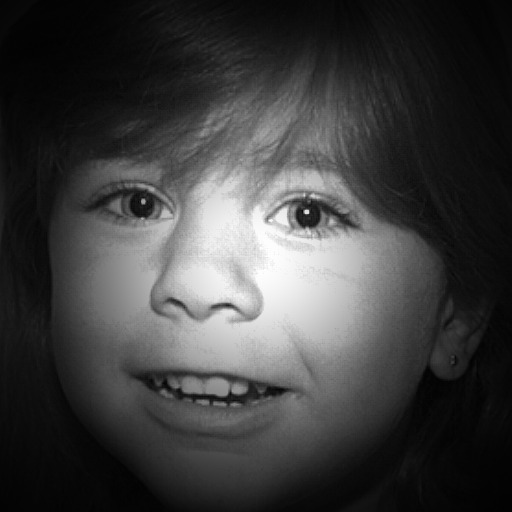
\includegraphics[width=0.1\textwidth]{../images/girl}
  & $\gamma_L=0.2$ & $\gamma_L=0.3$ & $\gamma_L=0.4$ & $\gamma_L=0.5$ & $\gamma_L=0.6$ & $\gamma_L=0.7$ \\
  $\gamma_H=1.2$
  & 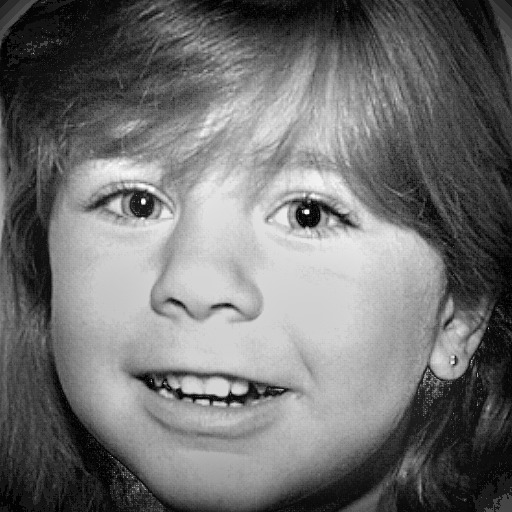
\includegraphics[width=0.135\textwidth]{../images/girl_2_12}
  & 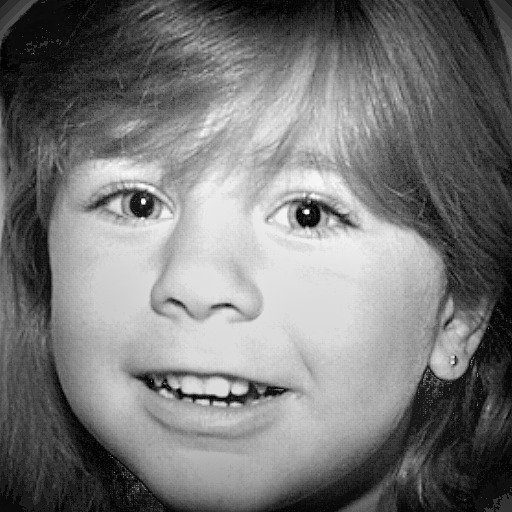
\includegraphics[width=0.135\textwidth]{../images/girl_3_12}
  & 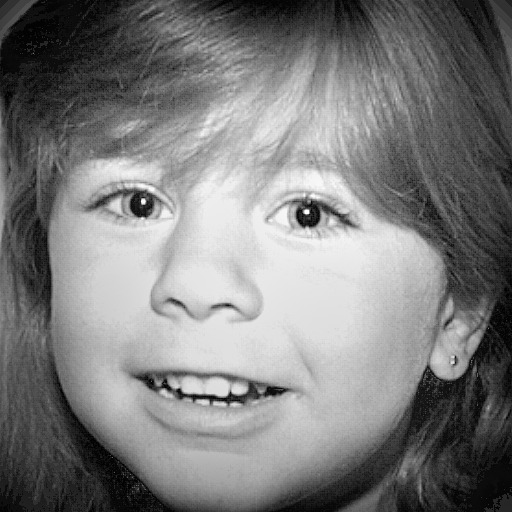
\includegraphics[width=0.135\textwidth]{../images/girl_4_12}
  & 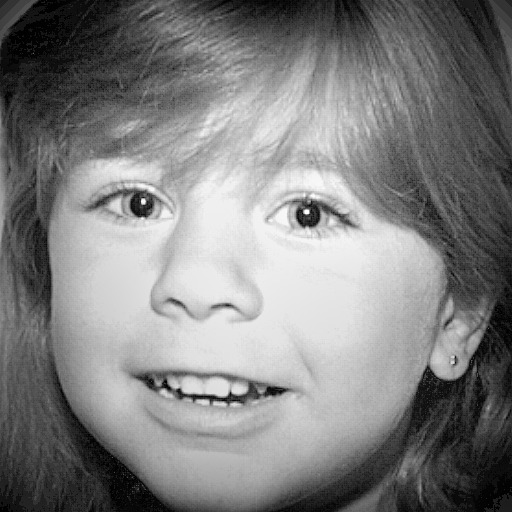
\includegraphics[width=0.135\textwidth]{../images/girl_5_12}
  & 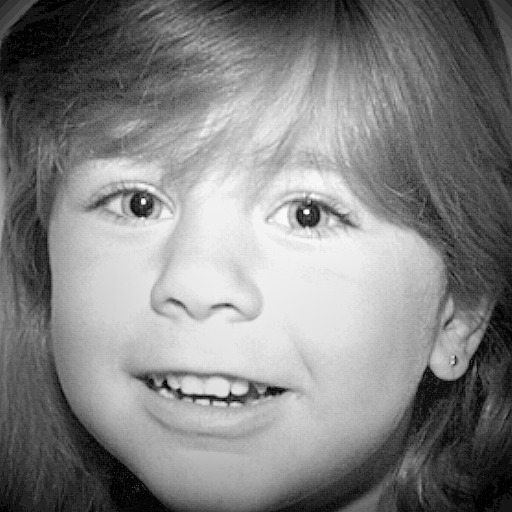
\includegraphics[width=0.135\textwidth]{../images/girl_6_12}
  & 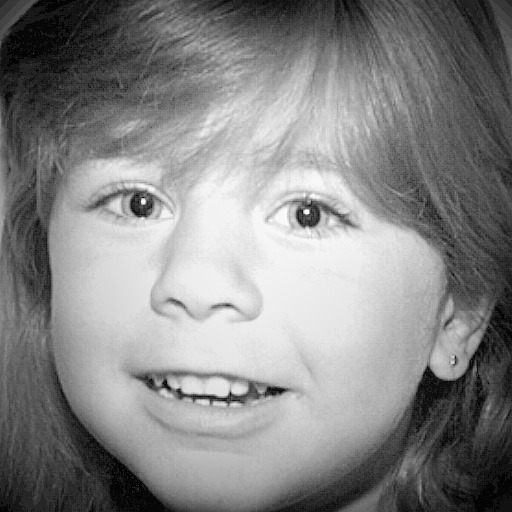
\includegraphics[width=0.135\textwidth]{../images/girl_7_12} \\ [-4pt]
  $\gamma_H=1.3$
  & 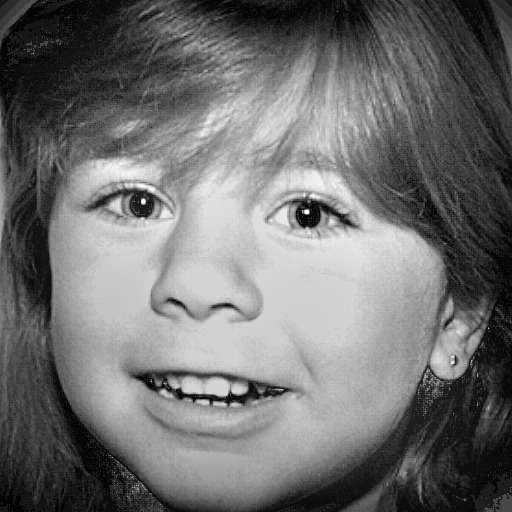
\includegraphics[width=0.135\textwidth]{../images/girl_2_13}
  & 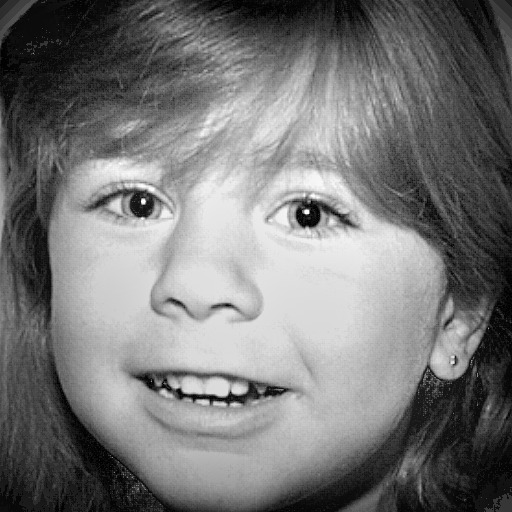
\includegraphics[width=0.135\textwidth]{../images/girl_3_13}
  & 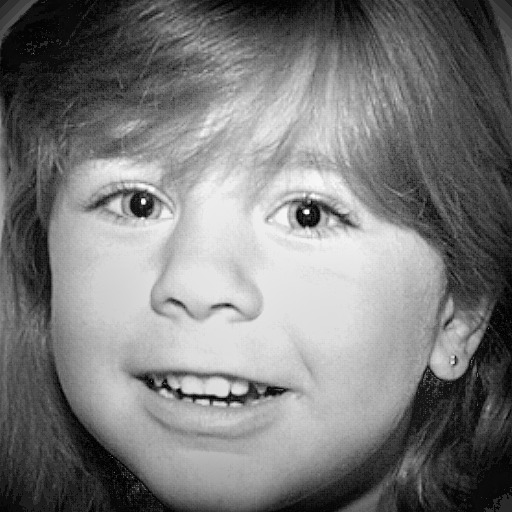
\includegraphics[width=0.135\textwidth]{../images/girl_4_13}
  & 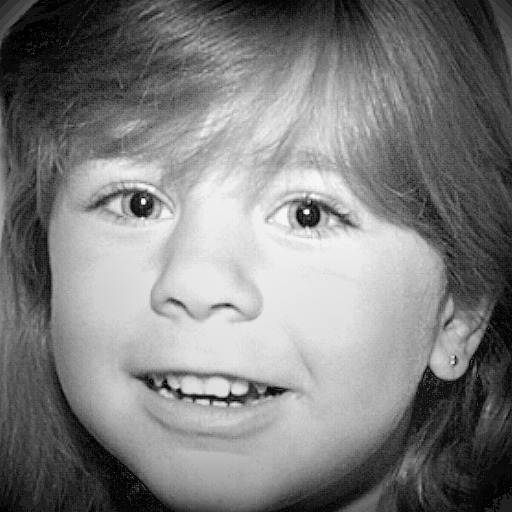
\includegraphics[width=0.135\textwidth]{../images/girl_5_13}
  & 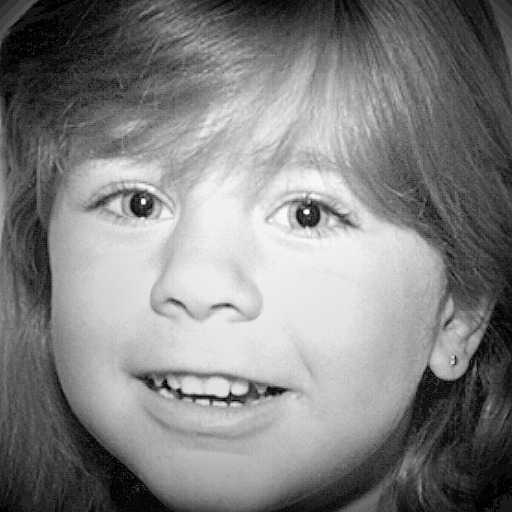
\includegraphics[width=0.135\textwidth]{../images/girl_6_13}
  & 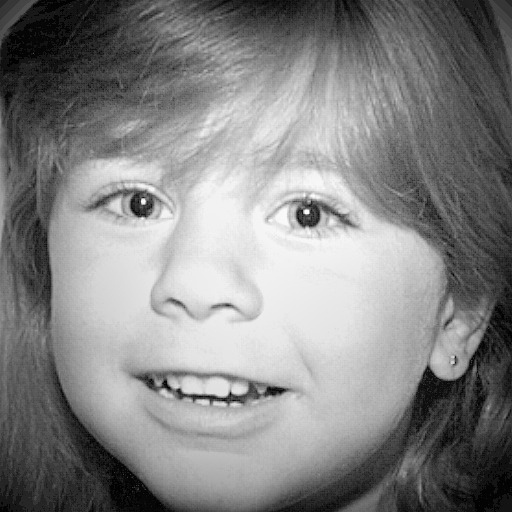
\includegraphics[width=0.135\textwidth]{../images/girl_7_13} \\ [-4pt]
  $\gamma_H=1.4$
  & 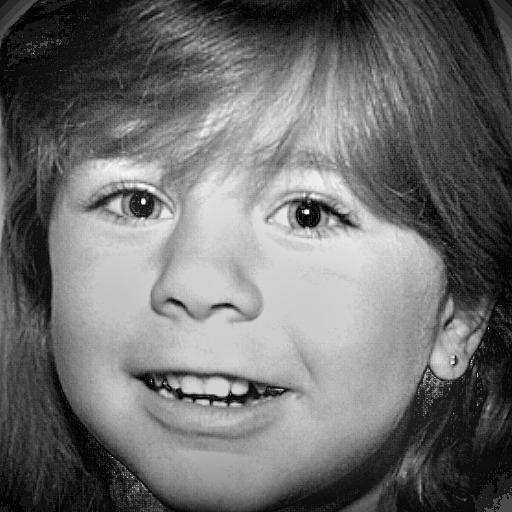
\includegraphics[width=0.135\textwidth]{../images/girl_2_14}
  & 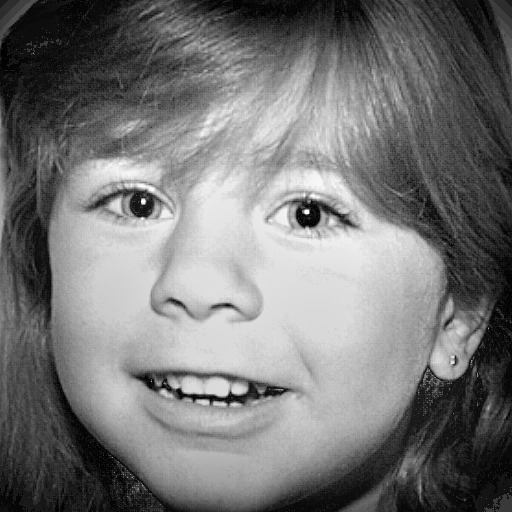
\includegraphics[width=0.135\textwidth]{../images/girl_3_14}
  & 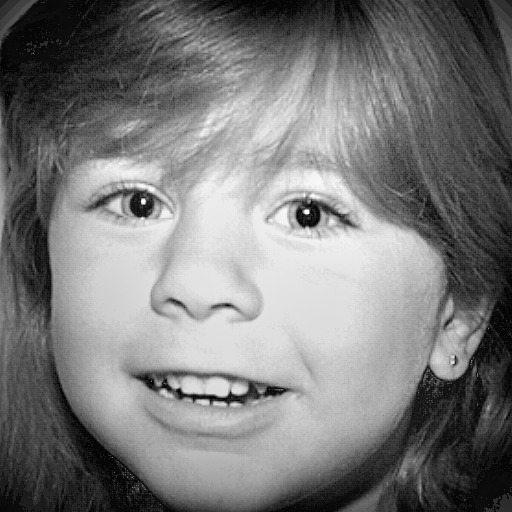
\includegraphics[width=0.135\textwidth]{../images/girl_4_14}
  & 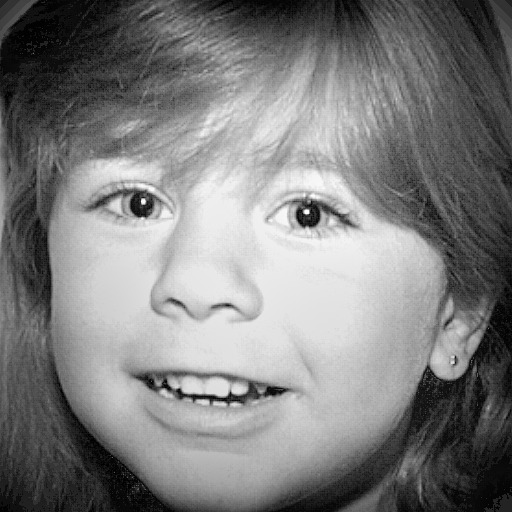
\includegraphics[width=0.135\textwidth]{../images/girl_5_14}
  & 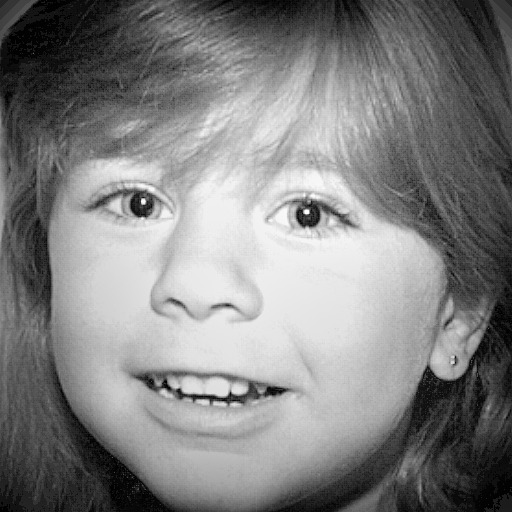
\includegraphics[width=0.135\textwidth]{../images/girl_6_14}
  & 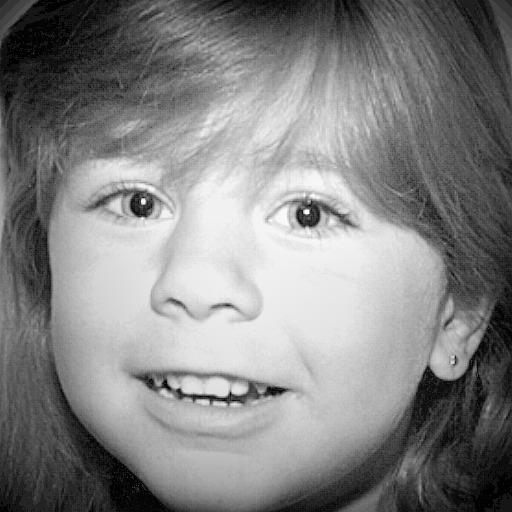
\includegraphics[width=0.135\textwidth]{../images/girl_7_14} \\ [-4pt]
  $\gamma_H=1.5$
  & 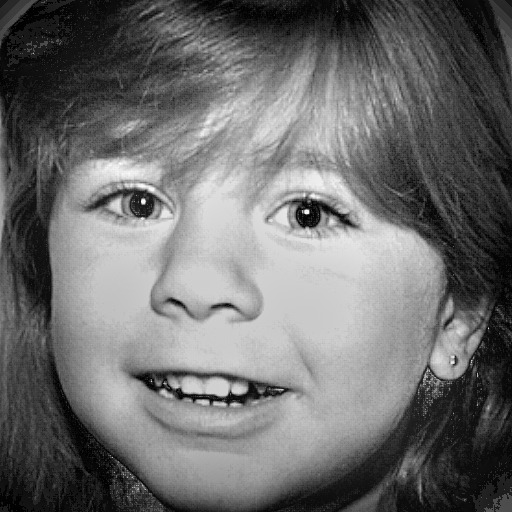
\includegraphics[width=0.135\textwidth]{../images/girl_2_15}
  & 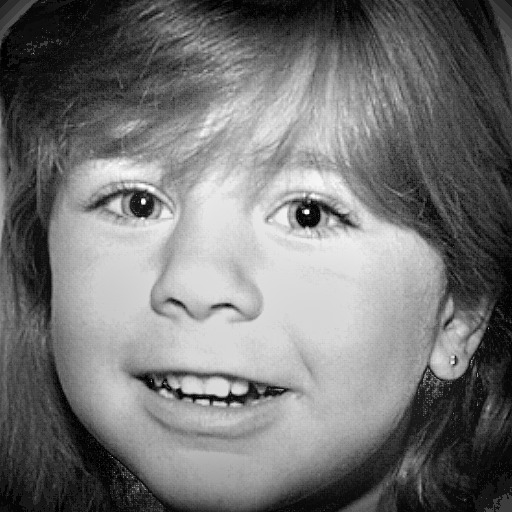
\includegraphics[width=0.135\textwidth]{../images/girl_3_15}
  & 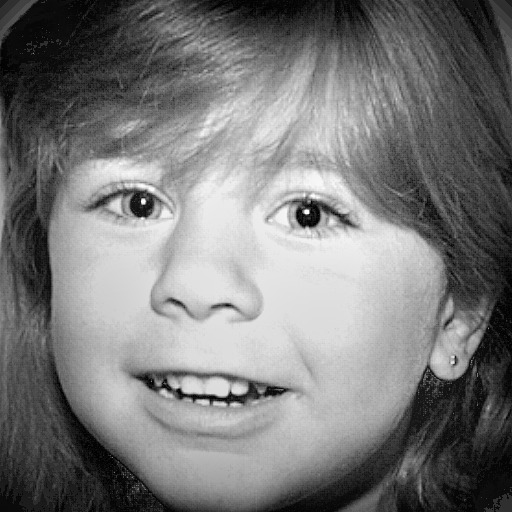
\includegraphics[width=0.135\textwidth]{../images/girl_4_15}
  & 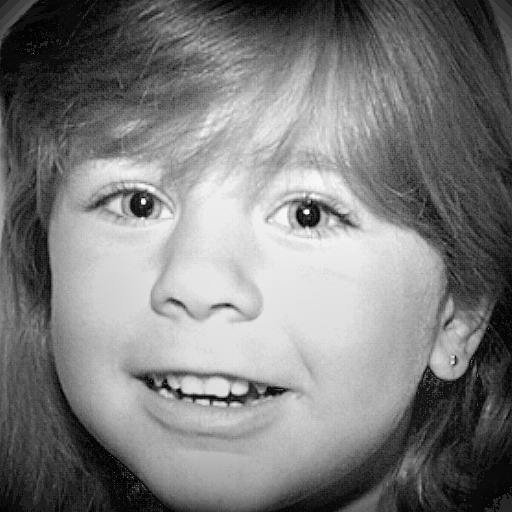
\includegraphics[width=0.135\textwidth]{../images/girl_5_15}
  & 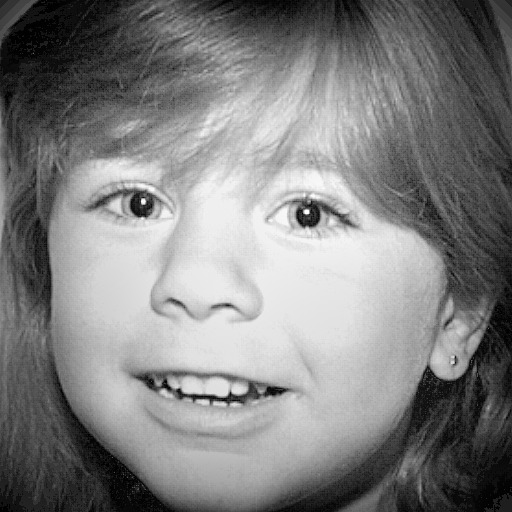
\includegraphics[width=0.135\textwidth]{../images/girl_6_15}
  & 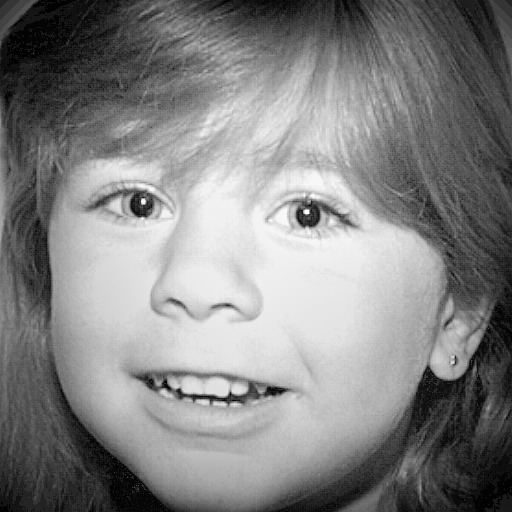
\includegraphics[width=0.135\textwidth]{../images/girl_7_15} \\ [-4pt]
  $\gamma_H=1.6$
  & 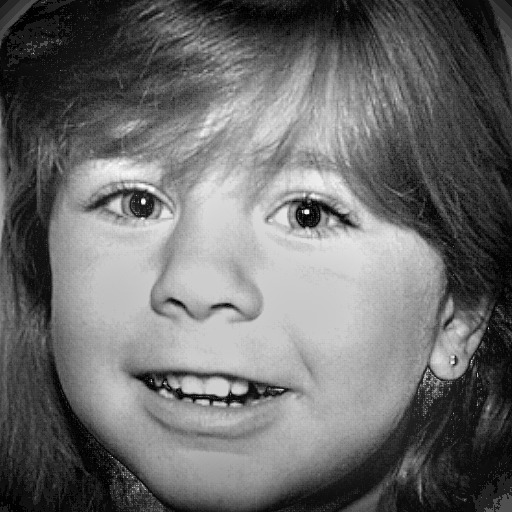
\includegraphics[width=0.135\textwidth]{../images/girl_2_16}
  & 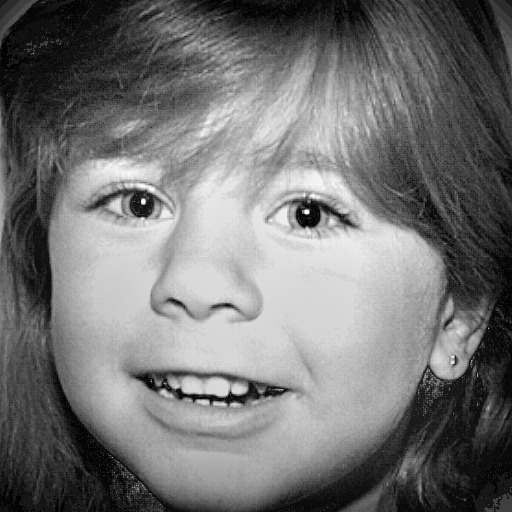
\includegraphics[width=0.135\textwidth]{../images/girl_3_16}
  & 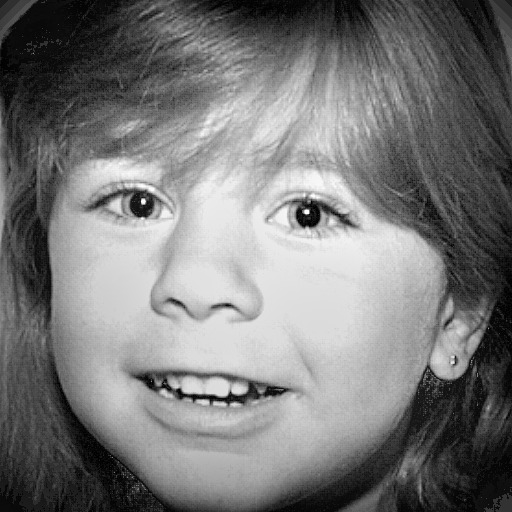
\includegraphics[width=0.135\textwidth]{../images/girl_4_16}
  & 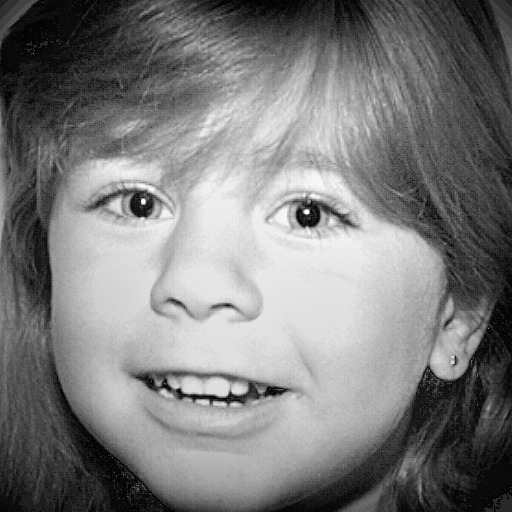
\includegraphics[width=0.135\textwidth]{../images/girl_5_16}
  & 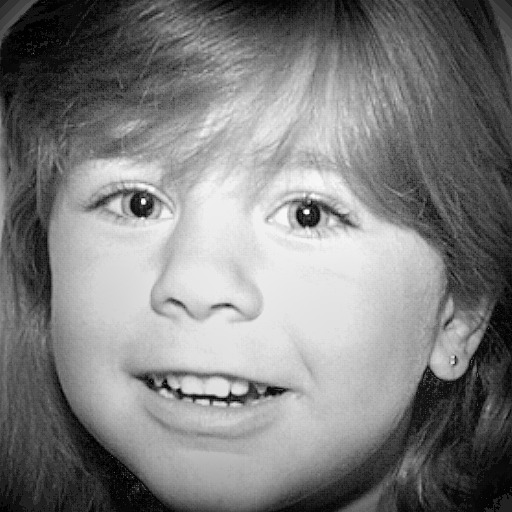
\includegraphics[width=0.135\textwidth]{../images/girl_6_16}
  & 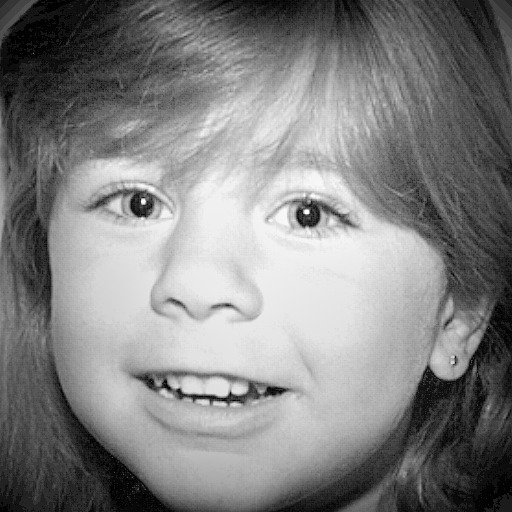
\includegraphics[width=0.135\textwidth]{../images/girl_7_16} \\ [-4pt]
  $\gamma_H=1.7$
  & 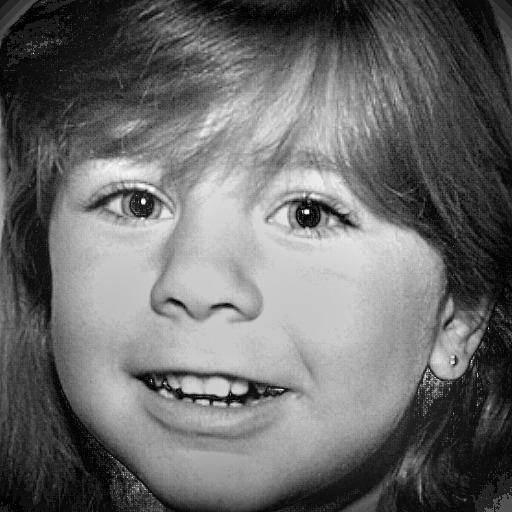
\includegraphics[width=0.135\textwidth]{../images/girl_2_17}
  & 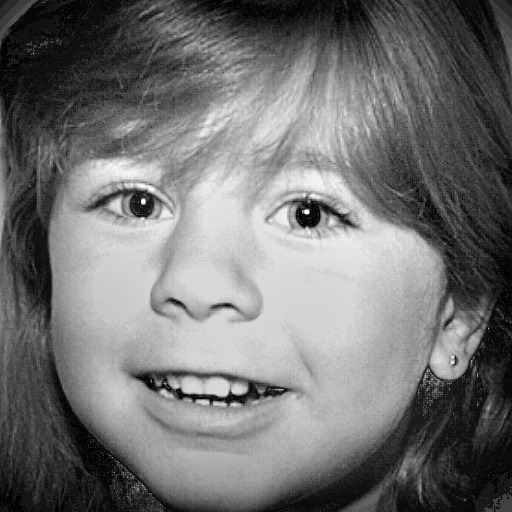
\includegraphics[width=0.135\textwidth]{../images/girl_3_17}
  & 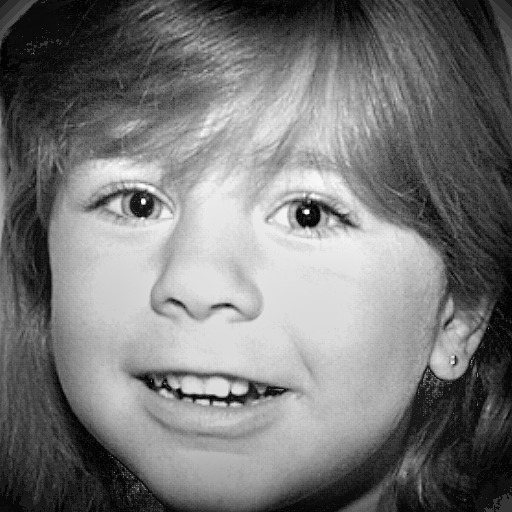
\includegraphics[width=0.135\textwidth]{../images/girl_4_17}
  & 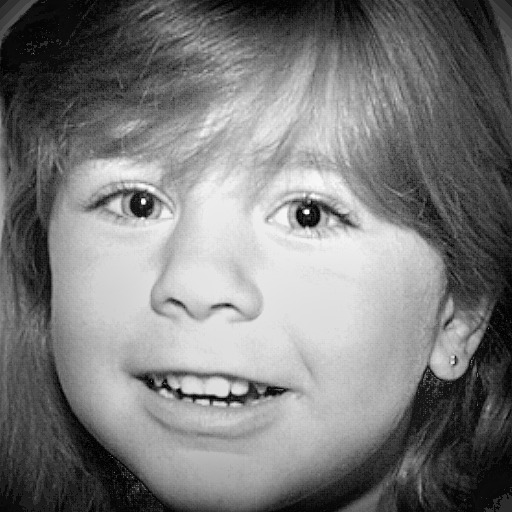
\includegraphics[width=0.135\textwidth]{../images/girl_5_17}
  & 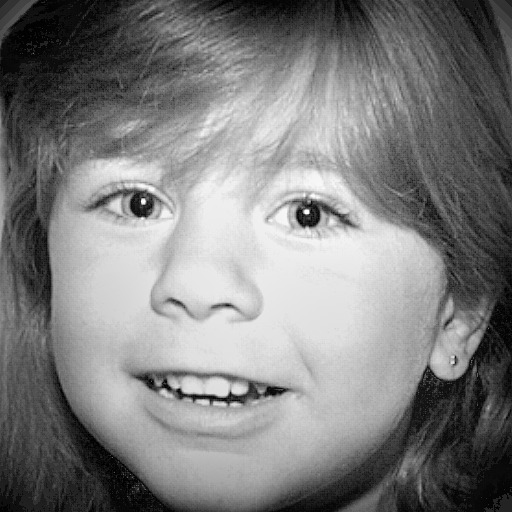
\includegraphics[width=0.135\textwidth]{../images/girl_6_17}
  & 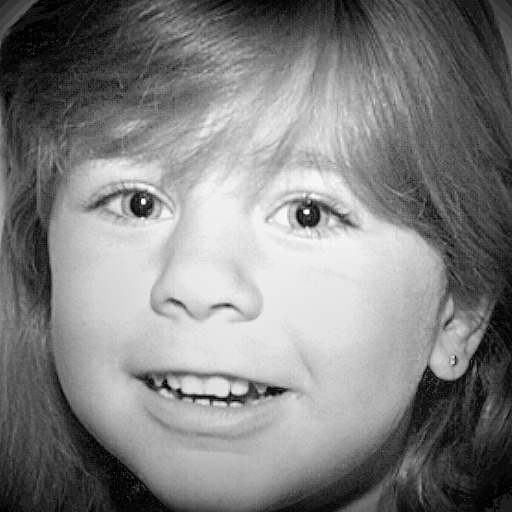
\includegraphics[width=0.135\textwidth]{../images/girl_7_17} \\ [-4pt]

  
\end{tabular}
\vfill

